\chapter{Statistiques}
%\stepcounter{module}

{\AlegreyaSansLight \large
\begin{center}
\textbf{Crédit :} 11 heures\\
\textit{4 heures hebdomadaires}
\end{center}
}

\minitoc

\section{Introduction}

\subsection{Présentation du module}
Ce module vise à rendre l'apprenant capable de traiter de façon réussie, des situations de vie de la famille  "organisation des données et estimation des quantités dans la consommation des biens et services ". Il s'agit pour lui de :
\begin{itemize}
\item Déployer un raisonnement mathématique pour identifier et formaliser des situations de vie qui se rapportent aux proportionnalités.
\item Résoudre des problèmes relatifs à des situations telles que le placement d'argent, la remise au cours d'achat divers, le partage proportionnel, la collecte et l'exploitation des données, les interprétations des résultats des enquête ....
\end{itemize}
Pour y parvenir, il est nécessaire de consolider et de renforcer les acquis sur les proportionnalités, les pourcentages et l'échelle vue en sixième tout en restant sur les habiletés cognitives que sont la connaissance, la compréhension et l'application.\\
Ce module est par excellence celui qui, à ce niveau d'étude, comporte les situations de vie les plus familières à l'élève.

\subsection{Contribution du module à la finalité et aux buts curriculaires}
Le module permet de développer les compétences transversales suivantes : le sens de la concision, l'esprit critique et l'organisation rationnelle des données. A terme, ces attitudes permettent à l'apprenant de s'assumer comme membre responsable d'une famille, en même temps qu'elles lui permettent d'opérer des choix
judicieux et autonomes, dans la production, la consommation des biens et services.

\subsection{Contribution du module au programme d'études et aux domaines de vie}
Ce module est un des maillons essentiels du programme de 5ème. Il est par excellence lui-aussi, le domaine d'intégration des mathématiques dans la vie quotidienne. Les situations de vie et les exemples de situations auxquelles il renvoie, de même que toutes les autres composantes du module pourront tout aussi bien
intervenir en physique, dans les sciences de la vie et de la terre, en géographie, et plus tard en psychologie et en économie, pour ne citer que ces disciplines-là. Il permet à ce niveau de dégager de manière implicite et même transversale l'importance de l'interdisciplinarité dans plus d'un domaine d'apprentissage.\\
La maîtrise de cette notion que ce module développe est de nature à doter l'apprenant d'outils essentiels dont il a besoin dans la vie pratique. Sa contribution dans la gestion du budget familiale est indéniable. Son implication dans la détermination des quantités justifie son importance dans la consommation des biens. Une bonne maîtrise des statistiques situées est un atout majeur dans la consommation des informations, et dans l'exploitation, l'analyse et l'interprétation des données à caractère économique ou social.

\section{Matrice}

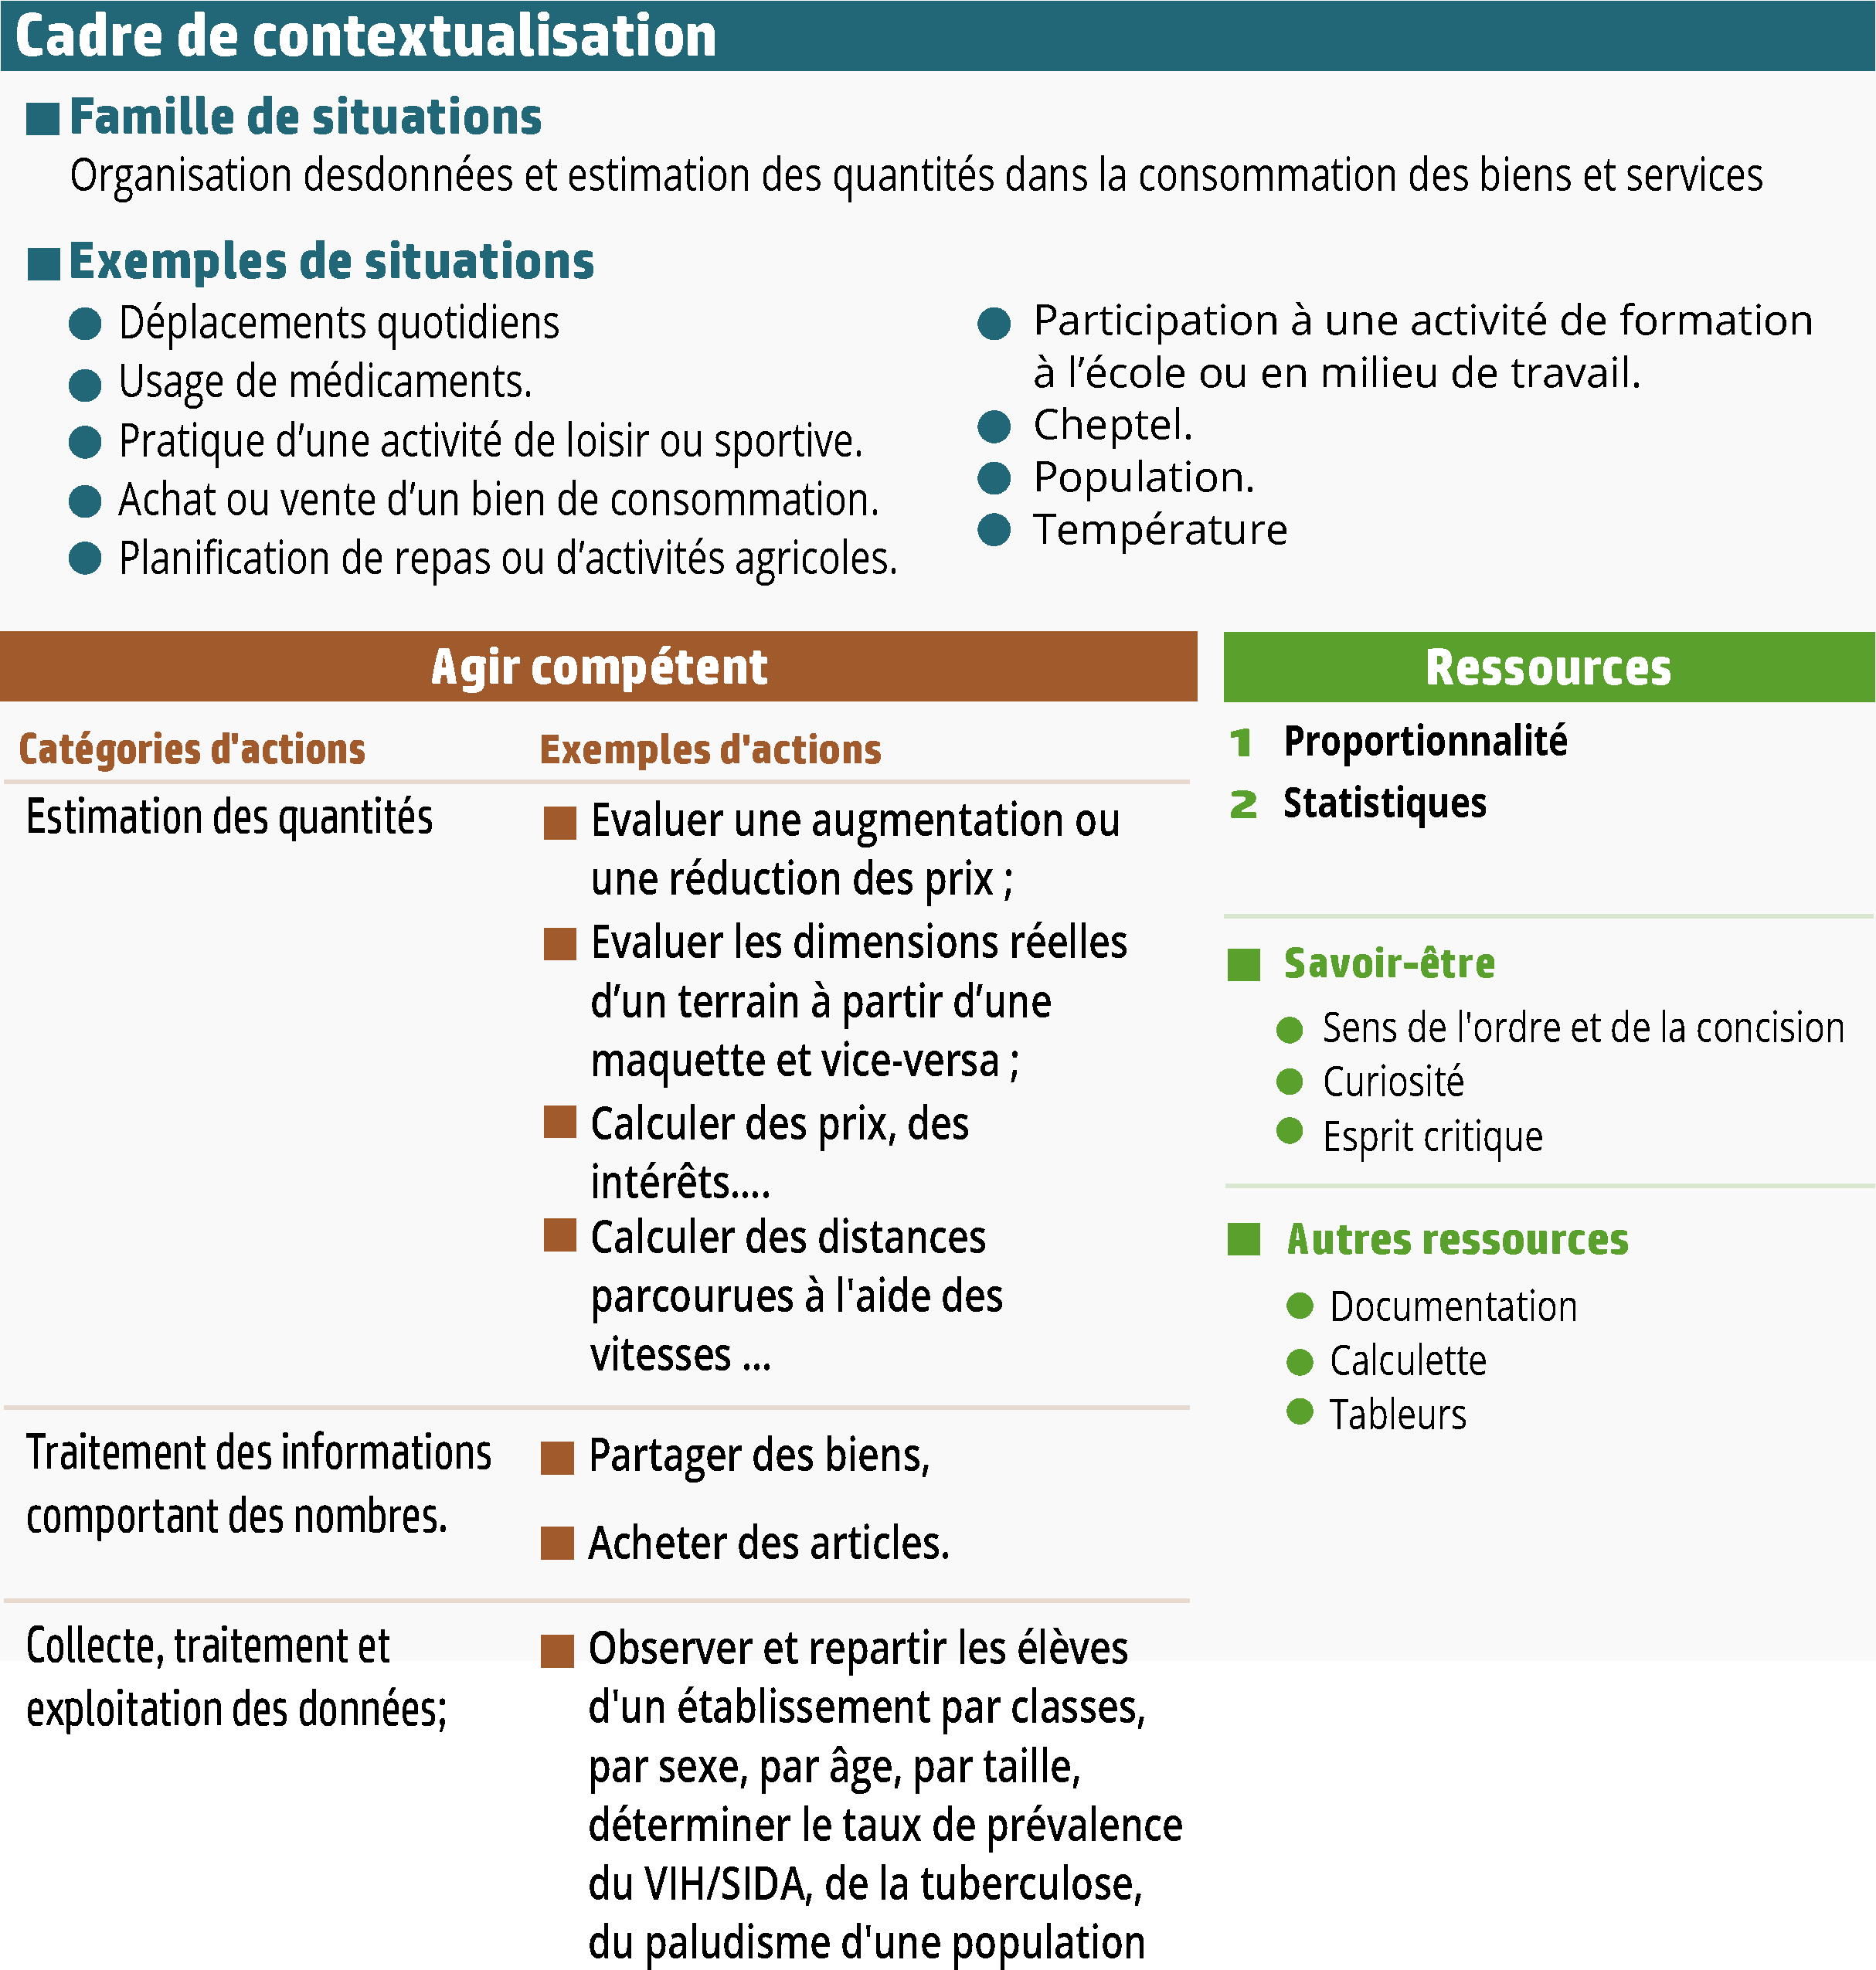
\includegraphics[width=\textwidth]{Module6.pdf} 

\subsection*{}
\addcontentsline{toc}{subsection}{\textbf{Ressource 1}: proportionnalité}
\ressource{Prop.pdf}

\savoir
\begin{itemize}
\item Coefficient de proportionnalité
\end{itemize}
\savoirfaire
\begin{itemize}
\item Calcul d'un coefficient de proportionnalité particulier : vitesse, masse volumique, débit.
\item Calcul d'un pourcentage, d'une échelle.
\item Représentation graphique d'une situation de proportionnalité dans un quadrillage.
\item Identification et exploitation du graphique d'une situation de proportionnalité dans un quadrillage.
\end{itemize}

\subsection*{}
\addcontentsline{toc}{subsection}{\textbf{Ressource 2}: statistiques}
\ressource{Stat.pdf}

\savoir
\begin{itemize}
\item \textit{Vocabulaire:} population, caractère, modalité, effectif d'une population, effectif d'une modalité.
\item Fréquences
\end{itemize}
\savoirfaire
\begin{itemize}
\item Elaboration d'un tableau des effectifs et des fréquences en pourcentage.
\end{itemize}